\usetikzlibrary{arrows.meta}
\begin{frame}<0>[fragile,label=storedXSS]{stored cross-site scripting}
\begin{tikzpicture}
    \node[draw,thick,inner sep=5mm,align=left,text=red!70!black,align=left] (commentBox) {
\begin{lstlisting}[language={}]
<script>
    document.location = 'http://attacker.com';
</script>
\end{lstlisting}
    };
    \node[anchor=south west] at (commentBox.north west) { Your comment: };
    \node[align=left,anchor=north west] (nameLabel) at (commentBox.south west) {
        Name: 
    };
    \node[draw,font=\tt,thick,inner sep=1mm,align=left,text=red!70!black,anchor=west,minimum width=5cm] at (nameLabel.east) {
        An Attacker
    };
\end{tikzpicture}
\end{frame}

\begin{frame}[fragile,label=storedXSS2]{stored cross-site scripting}
    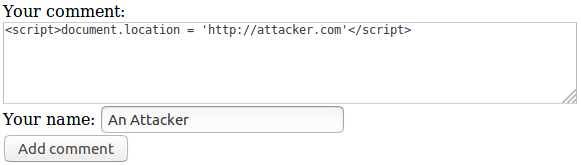
\includegraphics[width=\textwidth]{../web/stores-xss}
\end{frame}

\section{Web overall}

\begin{frame}{the web}
    \begin{tikzpicture}
        \node[draw,thick,fill=blue!30] (browser) {
            Web Browser
        };
        \node[draw,thick,fill=green!30,right=2cm of browser] (webSite1) {
            facebook.com
        };
        \node[draw,thick,fill=green!30,below=.5cm of webSite1] (webSite2) {
            foobar.com (uses facebook login)
        };
        \node[draw,thick,fill=red!30,below=.5cm of webSite2] (webSite3) {
            evil.com (run by attacker)
        };
        \draw[thick,Latex-Latex] (browser) -- (webSite1.west);
        \draw[thick,Latex-Latex] (browser) -- (webSite2.west);
        \draw[thick,Latex-Latex] (browser) -- (webSite3.west);
    \end{tikzpicture}
\begin{itemize}
    \item one web browser talks to multiple websites
    \item how does it (or does it) keep each websites seperate?
    \item even though websites can link to each other/etc.?
\end{itemize}
\end{frame}

\begin{frame}{the browser is basically an OS}
    \begin{itemize}
    \item websites are JavaScript programs
    \item websites can communicate with each other
        \begin{itemize}
        \item one website can embed another
        \item cause browser to send requests to another
        \end{itemize}
    \item websites can store data on the browser
        \begin{itemize}
        \item cookies
        \item local storage
        \end{itemize}
    \end{itemize}
\end{frame}

\subsection{HTTP}

\begin{frame}[fragile,label=HTTPReq]{HTTP requests}
\texttt{https://server.com/dir/file?query=string\#anchor} \\
    browser connects to server.com; \textbf{browser} sends:
\begin{framed}
\tt
\myemph<2>{GET}\tikzmark{method} /dir/file?query=string HTTP/1.1 \\
\myemph<3>{Host: \myemph<4>{server.com}\tikzmark{host}} \\
\myemph<3>{\textit{Other-Key}:  \textit{Other-Value}} \\
\ldots \\
~ \\
\end{framed}
    \begin{tikzpicture}[overlay,remember picture]
        \coordinate (overBox) at ([yshift=-2cm]current page.center);
        \tikzset{
            every node/.style={align=left,anchor=center},
        }
        \begin{visibleenv}<2>
        \node[my callout=method,anchor=center] at (overBox) {
            method: GET or POST most common \\
            GET --- read web page \\
            POST --- submit form
        };
        \end{visibleenv}
        \begin{visibleenv}<3>
        \node[my callout=host,anchor=center] at (overBox) {
            headers: \\
            extra information with request
        };
        \end{visibleenv}
        \begin{visibleenv}<4>
        \node[my callout=host,anchor=center] at (overBox) {
            example extra info: domain name from URL \\
            servers can host mutliple domains
        };
        \end{visibleenv}
\end{tikzpicture}
\end{frame}

\begin{frame}[fragile,label=HTTPResp]{HTTP responses}
\texttt{https://server.com/path/to/file?query=string\#anchor} \\
    after browser sends request; \textbf{server} sends:
\begin{framed}
\tt
HTTP/1.1 200 OK \\
Content-Type: text/html\tikzmark{contentType} \\
\textit{Other-Key}:  \textit{Other-Value} \\
~ \\
<html>\ldots
\end{framed}
    \begin{tikzpicture}[overlay,remember picture]
        \coordinate (overBox) at ([yshift=-2cm]current page.center);
    \end{tikzpicture}
\end{frame}

\begin{frame}{demo}
\end{frame}

\begin{frame}[fragile,label=HTMLForms1]{HTML forms (1)}
\begin{minted}[fontsize=\small]{HTML}
<form action="https://example.com/search/" method="GET">
<input type="hidden" name="recipient"
       value="webmaster@example.com">
Search for: <input name="q" value=""><br>
<input type="submit" value="Search">
</form>
\end{minted}
\begin{framed}
\tt\small
GET /search/?q=What\%20I\%20searched\%20for HTTP/1.1 \\
Host: example.com
\end{framed}
    \begin{itemize}
        \item q is ``\fbox{What I searched for}''
        \item \%20 --- character hexadecimal 20 (space)
    \end{itemize}
\end{frame}

\begin{frame}[fragile,label=HTMLForms2]{HTML forms (2)}
\begin{minted}[fontsize=\small]{HTML}
<form action="https://example.com/formmail.pl" method="POST">
<input type="hidden" name="recipient"
       value="webmaster@example.com">
Your email: <input name="from" value=""><br>
Your message:<textarea name="message"></textarea>
<input type="submit">
</form>
\end{minted}
\begin{framed}
\tt\small
POST /formmail.pl HTTP/1.1 \\
Host: example.com \\
Content-Type: application/x-www-form-urlencoded \\
~ \\
recipient=webmaster@example.com\&from=\textit{what\%20I\%20Entered}\\\&message=\textit{Some\%20message\%0a\ldots} \\
\end{framed}
\end{frame}

% FIXME: GET forms

\section{Trusting the client}

\begin{frame}[fragile,label=trustCli1]{trusting the client (1)}
\begin{minted}[fontsize=\small]{HTML}
<form action="https://example.com/formmail.pl" method="POST">
<input type="hidden" name="recipient"
       value="webmaster@example.com">
Your email: <input name="from" value=""><br>
Your message: <textarea name="message"></textarea>
...
<input type="submit">
</form>
\end{minted}
    \begin{itemize}
        \item if this my form, can I get a recipient of \texttt{spamtarget@foo.com}?
            \begin{itemize}
                \item Am I \myemph{enabling spammers}??
            \end{itemize}
        \item<2> Yes, because attacker could \myemph{make own version of form}
    \end{itemize}
\end{frame}
\begin{frame}[fragile,label=RefererHeader]{Referer header}
Submitting form at \texttt{https://example.com/feedback.html}:
\begin{framed}
\tt\small
POST /formmail.pl HTTP/1.1 \\
Host: example.com \\
Content-Type: application/x-www-form-urlencoded \\
\myemph{Referer: https://example.com/feedback.html} \\
~ \\
recipient=webmaster@example.com\&from=\ldots \\
\end{framed}
    \begin{itemize}
        \item \textbf{sometimes} sent by web browser
        \item if browser always sends, \myemph{does this help?}
    \end{itemize}
\end{frame}

\begin{frame}[fragile,label=trustCli2]{trusting the client (2)}
\begin{minted}[fontsize=\small]{HTML}
<form action="https://example.com/formmail.pl" method="POST">
<input type="hidden" name="recipient"
       value="webmaster@example.com">
...
<input type="submit">
</form>
\end{minted}
    \begin{itemize}
    \item can I get a recipient of \texttt{spamtarget@example.com} \myemph{and the right referer header}?
        \begin{itemize}
        \item attacker can't modify the form on example.com!
        \item browser sends header with URL of form
        \end{itemize}
    \item<2> Yes, because attacker can \myemph{customize their browser}
    \end{itemize}
\end{frame}

\begin{frame}[fragile,label=trustCliNoOne]{trusting the client (3)}
\setlength{\parskip}{0em}
\fontsize{10}{11}\selectfont\tt
ISS E-Security Alert  \\
February 1, 2000 

Form Tampering Vulnerabilities in Several Web-Based Shopping Cart Applications

\ldots

Many web-based shopping cart applications \myemph{use hidden fields in HTML forms} to
hold parameters for items in an online store. These parameters can include
the item's name, weight, quantity, product ID, and \myemph{price}.\ldots

\ldots

Several of these applications use a security method based on \myemph{the HTTP header}
to verify the request is coming from an appropriate site.\ldots

The ISS X-Force has identified \myemph{eleven shopping cart applications} that are vulnerable to form tampering. \ldots

~
\end{frame}

% FIXME: real client-side validation examples

